%%%%%%%%%%%%%%%%%  Debut du fichier Latex  %%%%%%%%%%%%%%%%%%%%%%%%%%%%%%
\documentclass[
    a4paper, 
    12pt, onecolumn,
    %draft
]{article}

%%% Pour un texte en francais
\usepackage[applemac]{inputenc}
\usepackage[T1]{fontenc}
\usepackage[francais]{babel}
	         % encodage des lettres accentuees
%\usepackage[utf-8]{inputenc}          % encodage des lettres accentuees
%\usepackage{graphicx}
%%\usepackage{graphicx} \def\BIB{}
\usepackage{multicol}
\usepackage{graphicx,wrapfig,lipsum} \def\BIB{}
\usepackage[pdftex]{hyperref}
\hypersetup{
    colorlinks,%
    citecolor=black,%
    filecolor=black,%
    linkcolor=black,%
    urlcolor=blue     % can put red here to visualize the links
}


%%% Quelques raccourcis pour la mise en page
\newcommand{\remarque}[1]{{\small \it #1}}
\newcommand{\rubrique}{\bigskip \noindent $\bullet$ }

\begin{document}

%%%%%%%%%%%%%%%%%%%%%%%%%  PREMIERE PAGE %%%%%%%%%%%%%%%%%%%%%%%%%%%%%%
%%% DANS CETTE PAGE, ON REMPLACE LES INDICATIONS ENTRE CROCHETS [...]
%%% PAR LES INFORMATIONS DEMANDEES
%%%%%%%%%%%%%%%%%%%%%%%%%%%%%%%%%%%%%%%%%%%%%%%%%%%%%%%%%%%%%%%%%%%%%%%

 
\noindent GENCI\hfill \textsc{Demande d'Attribution de Ressources Informatiques}

\begin{center}
\Large  \bf
Scientific description of the project
\end{center}
\bigskip

\rubrique Title of the project : {\bf Numerical simulations of wind-accretion in \underline{high mass X-ray (HMBX) binary systems} }
%Numerical simulation of Quasi-Periodic Oscillations in microquasars and comparison with observations

\rubrique  {\sc dari} number :
\hfill
%%% METTRE ICI LE RENSEIGNEMENTS DEMANDE
[Num\'ero de projet]

\rubrique  Scientist in charge : 
\hfill
%%% METTRE ICI LES RENSEIGNEMENTS DEMANDES
E{\sc l mellah} Ileyk


\rubrique Laboratory :  
\hfill
%%% METTRE ICI LES RENSEIGNEMENTS DEMANDES
AstroParticule \& Cosmologie (APC) - Paris 7


%%% HEURES DEMANDEES
\rubrique  Number of hours required (mono-process {\sc cpu}) :
   %%% DECOMMENTER LES LIGNES QUI CONCERNENT LE PROJET
   %%% ET REMPLACER [1200] PAR LE RENSEIGNEMENT DEMANDE
   %%% NE METTRE QUE LES DONNEES NON-NULLES
   % \newline CCRT  BULL IA64 Platine  : \hfill  [1200] heures scalaires
   % \newline CCRT  NEC SX8R Mercure   : \hfill [1200] heures vectorielles
   % \newline CCRT  BULL X\'eon Titane : \hfill [1200] heures scalaires
   % \newline CCRT  BULL X\'eon Titane : \hfill  [1200] heures CPU/GPU
   % \newline CINES IBM SP Hera        : \hfill  [1200] heures scalaires
   %  \newline CINES SGI ICE Jade       : \hfill  300\ 000 heures scalaires
   % \newline IDRIS IBM SP Vargas      : \hfill  [1200] heures scalaires
   % \newline IDRIS IBM BG/P Babel     : \hfill  [1200] heures scalaires
   % \newline IDRIS  NEC SX8 Brodie     : \hfill  [1200] heures vectorielles
     \newline CINES BULL Occigen      : \hfill  300\ 000 scalar hours

%%% RESUME
\section{Abstract}

%%% A COMMMENTER LORS DE LA REDACTION DU PROJET
%\emph{Longueur typique de {\bf 15 lignes}, longueur maximale de {\bf 1 page}.}

%The advent of high energy observation facilities in the last decades has proven the existence of powerful mechanisms emitting photons up to gamma-rays. 
%It is now commonly admitted that the most energetic events are associated with compact objects believed to be relics of massive stars. 
%These objects are prone to the most extreme gravity fields and are likely efficient attractors of the plasma present in their vicinity. 
%The motion of plasma in the close neighborhood of compact objects is only properly described in the framework of general relativistic magnetohydrodynamic (GR- MHD). 
%The equations governing GR-MHD are so complex that the only way to solve them is trough large-scale numerical simulations. 
%The topic of the present demand,  $200\ 000$ h CPU on the parallel CINES computer \lq Jade\rq\ , 
%is to sustain a computational effort dedicated to GR-(M)HD simulations of accretion flows near compact objects and to link them to synthetic observations of the 
%associated violent events.

\indent Our team is asking for  $300\ 000$ h-CPU on the parallel CINES supercomputer \lq Occigen\rq\ so as to investigate phenomenological statements concerning wind accretion in Supergiant High Mass X-ray Binaries (Sg-{\sc hmxb}), either {\bf hosting} a neutron star or a black hole. We developed a specific approach to described {\bf both} the large scale ballistic behavior of the stellar wind and the accretion radius of the compact object ({\bf whose ratio is typically of the order of 10}) and then, down to a few hundreds of gravitational radii of the compact object ({\bf whose size ratio to the accretion radius ranges from $10^{-3}$ to $10^{-5}$}). The huge dynamical spatial scale is made possible thanks to {\bf both} the highly parallelized {\sc MPI}-{\sc AMRVAC} software and  a stretched grid {\bf centered} on the compact object. The former code {\bf enables us} to grasp both shocks and non axisymmetric instabilities likely to give birth to potentially transient accretion discs around the compact object. {\bf The three-dimensional characterization of such flows} is a crucial prerequisite to better appreciate both the {\bf expected }X-ray time variabilities and the initial conditions from which close-in accretion discs ought to be modeled. \\

\newpage\section{Scientific motivation}

%%% A COMMMENTER LORS DE LA REDACTION DU PROJET
%\emph{Longueur typique {\bf 2 pages}, longueur maximale de {\bf 4 pages}. Si le projet se d\'ecompose en sous-projets, {\bf 2 pages additionnelles maximum par sous-projets}.}
%\vskip 0.2cm  
%\emph{Cette partie doit montrer l'int\'er\^et scientifique du projet. Le canevas suivant est propos\'e : 
%pr\'eciser les objectifs,
%situer les travaux de l'\'equipe sur le th\`eme de recherche propos\'e tant vis \`a vis du travail d\'ej\`a  
%effectu\'e par l'\'equipe (r\'esultats acquis sur le sujet), que vis \`a  vis d'autres travaux sur un plan national
%et international,
%donner une liste de publications de l'\'equipe dans le domaine dans la section \ref{Sec:Biblio}. On peut joindre au dossier tous les documents (en format pdf) annexes jug\'es utiles.}

\indent The number of detected Sg-{\sc hmxb} has dramatically increased as the recent space missions stretched the limits of the high energy part of the light spectrum (e.g. L{\sc iu} et al 2006). Once believed to be rare (I{\sc llarionov} \& S{\sc unyaev} 1975), those X-ray luminous wind-fed compact objects orbiting an evolved {\sc O}/{\sc B} star {\bf did not fit into} the previously sketched categories. The characterization of the companion star is usually a {\bf challenge} in itself because of the high obscuration {\bf occurring} in those systems lying close from the galactic plane {\bf several} kiloparsecs away from us. {\bf Hopefully}, the recent {\bf discovery?}  of {\sc hmxb} {\bf outside of the galactic plane} partly lifted this difficulty. Still, the main information we get from those objects (some being microquasars whom study is believed to enrich our understanding of Active Galactic Nuclei) comes from the X-ray emission to which they owe their name.\\

\indent This hard radiation, {\bf discovered} in 1962 (G{\sc iacconi} et al 1962), brought up so many questions that {\bf it} remains puzzling when one attempts to explain the different "families" of behaviors observed - if that an agreement is found on the very classification. Those complex systems have been dissected (the launching of the stellar wind, its orbital trajectory, the shocks it can form, its subsequent accretion onto the compact objects, etc) but {bf in order} to go beyond toy-models, one needs to tackle the entire {\bf dynamics} of the stellar material, from the clumpy wind scale down to the {\bf close vicinity of} the compact object ({\bf being in our study around a hundred gravitational radii of a black hole or the magnetosphere radius of a neutron star}). For instance, being able to corroborate the identity of the compact object deduced from orbital considerations would bring more scientific {\bf weight} to the current observational constraints on the equation of state of matter in neutron stars. {\bf  In order to achieve such assessment}, one must first wonder how the orbital parameters (orbital period, mass of the compact object, masses ratio, eccentricity) and the properties of the stellar companion (wind velocity, {\bf ejection} mass rate {\bf and} clumpiness) {\bf influence} the compact object environment {\bf in order} to disentangle the contingent from the essential causes. Independently from the accreting body nature, the systems we intend to model already differ a lot from each other :\\
\begin{itemize}
\item \textbf{Cyg X-1 :} it hosts a highly R{\sc oche} lobe deformed (A{\sc vni} et al 1975) Sg star (S{\sc henavrin} et al 2011) orbiting a compact object of comparable mass every 5.6 days. Although one of the most studied {\sc hmxb} - if not the most - its genericity remains suspicious.\\
\item \textbf{LMC X-1 :} this extragalactic close X-ray binary presents a peculiar Onfp class (W{\sc alborn} et al 2010) star whom rapid rotation might transfer an important amount of stellar angular momentum to the wind. \\
\item \textbf{Vela X-1 :} the archetype of the Sg-{\sc hmxb}. Characterized by a larger mass ratio than the two previous ones, this eclipsing system feeds its compact object through the specially intense stellar wind of its B stellar companion, well embedded in its R{\sc oche} lobe.\\
\item \textbf{4U 1907+09 :} in this high mass ratio eccentric X-ray binary, a hybrid accretion might proceed, mixing R{\sc oche} lobe overflow and wind accretion. The torque accreted matter exerts on the compact object has been reported to potentially alternate between positive and negative values.\\
\end{itemize}

\begin{wrapfigure}{l}{6cm}
%\caption{A wrapped figure going nicely inside the text.}
\vspace*{-10pt}
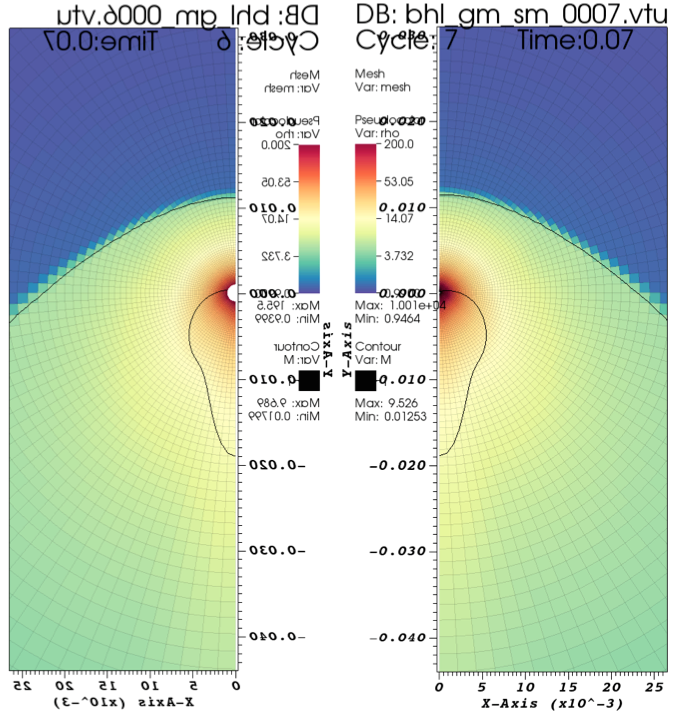
\includegraphics[height=7cm, width=6cm]{shock_independent_inner_boundary_size}
\caption{Bow shock and sonic surfaces of an axisymmetric 2.5D accretion flow for two different accretion size.}
\label{fig:bow2.5d}
\end{wrapfigure} 

\indent B{\sc ondi}, H{\sc oyle} and L{\sc yttleton} {\bf laid} the foundations of an understanding of axisymmetric accretion flows (see a review by E{\sc dgar} 2004) like the one we started from as a numerical sanity check (see next paragraph). Their ballistic approach has been improved to account for pressure effects (H{\sc oredt} 2000), making the accretion line in the wake of the accreting body an accretion tail. In the end of the 1980's, two dimensional simulations of those flows (M{\sc atsuda} 1987, F{\sc ryxell} \& T{\sc aam} 1988) revealed an instability, coined {\bf as} the flip-flop one ; the two dimensional cylindrical geometry, the low resolution and the oversized inner boundary compare to the actual size of the accretor made this instability suspicious to the community, until theoretical models (F{\sc oglizzo} et al 2005) supported the possibility of an instability growth important enough to account for the formation of tiny and transient discs around the accretor. The issue has remained polemical up to nowadays as the computational capabilities have proven insufficient to grasp the whole problem. That is why we developed a reliable upwind scheme on a logarithmic three dimensional grid centered on the accretor to jump from large to small scales at a cheaper computational cost. However, this numerical swindle would not have been enough to beat the dynamics barrier without the highly parallelized structure of the finite volumes program {\sc mpi}-{\sc amrvac}. Using the two together, we have now good hope to make the inner boundary small enough to be whether physical (for neutron star systems) or transparent (for black hole systems). The Figure\,\ref{fig:bow2.5d} shows for instance a simulation where the structure of the flow and of the sonic surface is not altered by the unphysical inner boundary.\\

 \begin{figure}[h]
 \centering
 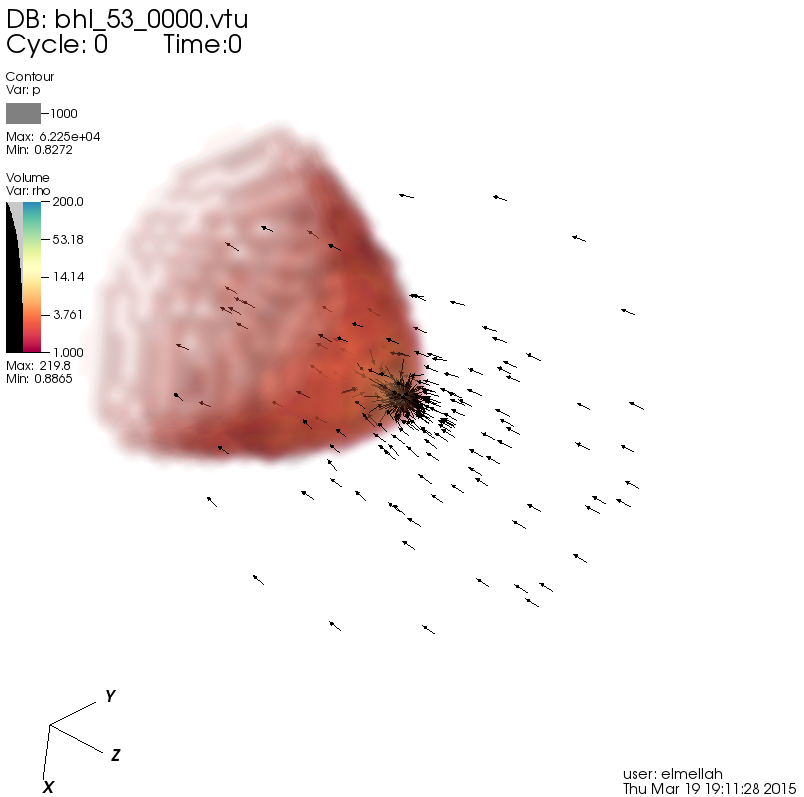
\includegraphics[width=9cm]{3D_initial_setup}  
 \caption{3D initial setup deduced from the relaxed 2.5D one}
 \end{figure}
 
\indent Concerning the numerical reliability of our setup, we already validated the behavior of the gas in 2.5D {\bf spherical geometry} within the accretion radius by showing that the axisymmetric configuration is in agreement with semi-analytical results derived by F{\sc oglizzo} \& R{\sc uffert} (1997), especially {\bf regarding} the topology of the sonic surface for a detached bow shock. {\bf Nevertheless}, {\bf in order to} enable non axisymmetric instabilities to develop, one needs to consider more realistic outer boundary conditions. We  {\bf then} need to {\bf lift the 2.5D assumption} and go for a full 3D configuration. The required computational time motivates our application to the {\sc cines} facility.\\
\indent {\bf It is noteworthy that} our work also aims to help constraining future and incoming observational mission (\href{http://www.the-athena-x-ray-observatory.eu}{{\sc athena}} \& \href{http://astro-h.isas.jaxa.jp/en/}{{\sc astro-h}} eg) : which waveband should we look after? Which time scale should we aim to characterize processes involved in the building up of an accretion disc? Since the mass accretion rate determines the available power convertible into X-ray luminosity, such simulations would also set lower limits for the sensibility required to probe events taking place in the very neighborhood of the compact object. The related studies, led in parallel, of the instabilities in this strong gravitational field regimes (e.g. the {\sc nova}s project) might, one day, tell us more about the physics at stake in those extreme environments : what kind of hitherto unseen events can take place in the wildness of a neutron star light cylinder or of a black hole ergosphere?
\begin{table}[h]
\centering
\begin{tabular}{||c|c|c||}
\hline\hline
Nom et pr\'enom & Fonction & Etablissement \\\hline
EL MELLAH Ileyk & Doctorant & APC\\ \hline 
CASSE Fabien & Ma\^itre de conf�rences & APC \\ \hline
DODU Fabrice & Ing\'enieur de recherche &APC \\ \hline
\hline\hline
\end{tabular}
\caption{Members of the collaboration}
\end{table}
\section{Presentation of the numerical tools}

%%% A COMMMENTER LORS DE LA REDACTION DU PROJET
%\emph{Cette partie doit \^etre suffisamment pr\'ecise et argument\'ee pour permettre au Comit\'e Th\'ematique d'appr\'ecier 
%l'ad\'equation de l'architecture
%pr\'evue (scalaire, vectorielle ou parall\`ele, GPU ...) au probl\`eme pos\'e. Il convient aussi de justifier clairement la n\'ecessit\'e de l'utilisation d'un tr\`es grand \'equipement pour le traitement informatique du projet.
%Voici une proposition de plan (\`a adapter selon le sujet) :
%Algorithme utilis\'e, adaptation \`a la plate-forme vis\'ee; Modalit\'es d'optimisation (vectorisation, optimisation superscalaire, parall\'elisation); Structure du programme; Logiciels n\'ecessaires; Langages utilis\'es; Biblioth\`eques pr\'evues; Syst\`emes de gestion de bases de donn\'ees ou syst\`emes documentaires utilis\'ees.}


\subsection{Numerical methods and setup}

%%% A COMMMENTER LORS DE LA REDACTION DU PROJET
%\emph{Longueur typique de  {\bf 4 pages}, longueur maximale de {\bf 6 pages}.}

\subsubsection*{{\sf AMRVAC} code}

The code {\sf AMRVAC} is an adaptative mesh refinement code parallelized with MPI. This code was created to be used in a wide
variety of physical applications that can be described by a set of conservative equations, independently of their nature (and not
only fluides).  Among the pre-existing physics modules there are modules to see the hydrodynamical and MHD equations in the classical
or special relativity case.
Several types of solver are also implemented, for example TVD Lax-Friedrich or HLL solvers. \newline
The AMR grid structure is based on the use of sub-grids (of a few tens of cells in every dimension) in a tree architecture (octree in 3D).
At each iteration the code uses an internal (Lohner's method)  or user-supplied criteria to determine if a sub-grid needs
to be refined, left as it is, or unrefined. The tree structure replaces each refined sub-grid by a $2^D$ sub-grid of the same cell-size but with 
the area of each cell less by a factor $2^D$. {\bf For the present project, we do not use the adaptative mesh refinement but instead we designed a non-regular grid fitting the geometry of the system and enabling us to reach outer radius to inner radius ratio up to $10^5$ at a low computational cost. The grid is designed to maintain the same radial to azimuthal cell size ratio constant for any radius of the simulation (Ileyk tu pourrais montrer un exempt de grille). The smallness of the cells close to the inner boundary sets CFL time step so small that several tens of millions of iterations are expected in order to describe the flow dynamics. Such computation can only be achieved using a large number of CPUs available on supercomputers.}
\newline

The parallelization is done with MPI and the scalability test done on \lq Jade\rq  by Z. Meliani showed an efficiency of 
the order of 80\% on 2000 processors. This value is very close to the theoretical limit when one takes into account the I/O of the code 
needed to write the data. Those results of the parallelization efficiency were obtained using a test case in relativistic hydrodynamics, 
taking into account the propagation of shocks with Lorentz factors between 100 and 1000. The main test was done in 2D with 10 levels of AMR
with a refinement ratio of 2. This allowed us to locally increase the resolution of the simulation by a factor of $218$.
% on the last level compare to the initial level.
 \begin{figure}
\centering
 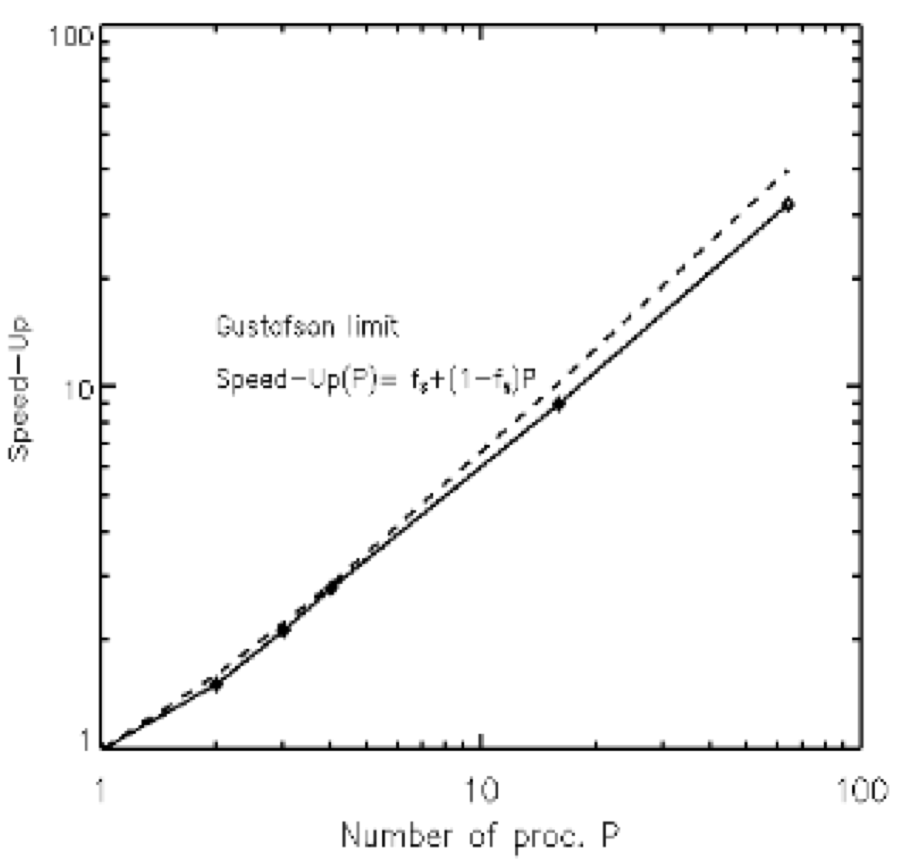
\includegraphics[width=8cm]{scaling_1} 
 \caption{Scaling of the MPI-AMRVAC code performed on the JADE super-computer.} 
\end{figure}
The {\sf MPI-AMRVAC} code also includes two different methods to write the data allowing a better flexibility. Indeed,
{\sf MPI-AMRVAC} can either use the method  MPI-II/IO or the method that consists of sending all the data from the slave node to the master node
to minimise the number of processors taking part in the writing.



\subsection{Justification du temps}

    We ask for a relatively small quantity of computing time (100\ 000h)  that will be shared between all the members of our groups
    since we are still in an early  stage of our project and cannot foresee all issues that will have to be fixed during the GR-MHD development.
    This amount of computational time will allow us to perform about $30$ runs on 128 processors, mainly devoted to the study of hydrodynamical accretion disks in the very close vicinity of black holes with various spin factors. We will also dedicated a part of these simulations to the study of the birth of Rossby Wave instability near the last stable orbit of the disk. The expected variability of the emission spectra (calculated with the GYOTO code) will be compared to observations from micro quasars where quasi-periodic oscillations are observed. 
    If we make faster progress than anticipated we intend to resubmit a proposal in june 2014. 

%une simulation en moyenne se compte en jour, avec  entre 64 et 512 proc...
%   256 proc pendant 24h: 5000...   
%   donc 10jours de simu, a notre niveau actuel va nous permettre d'avancer... et si besoin redemande en juin
%   


%\subsection{Justification de l'emploi de la machine demand\'ee}

%%% A COMMMENTER LORS DE LA REDACTION DU PROJET
%\emph{Longueur typique de {\bf 1 page}, longueur maximale de  {\bf 2 pages}.}

%GYOTO can be run under Linux or Mac OS X. It needs the following dependencies: xercesc-3 (to handle XML input �les) and cfitsio2 (to handle FITS output �les).

\newpage\section{Bibliographie}
\label{Sec:Biblio}
%\emph{Dans cette partie, identifier les articles de l'\'equipe par rapport \`a la bibliographie g\'en\'erale}
%\emph{Par exemple: Les r\'ef\'erences \protect\cite{My_paper:2009} sont celles de l'\'equipe.}

%\bibliographystyle{plain}
%\bibliography{/Users/vast/A_PHYSIQUE/biblio/mybiblio}
%\begin{thebibliography}{1}
%
%%%bibitem{BH} Balbus, S.A.; Hawley, J. F., 1991, ApJ, 376, 214.
%
%%%\bibitem{M10} Meheut, H.; Casse, F.; Varniere, P.; Tagger, M., 2010, A\&A, 516, 31.
%
%\bibitem{K11} R. Keppens, Z. Meliani, A.J. van Marle, P. Delmont, A. Vlasis, \& B. van der Holst, 2011, JCP. Full paper,  
%Accepted for special topical issue, with R. Keppens as Associate Editor. 
%
%%%\bibitem{R02} Rodriguez, J.; Varniere, P.; Tagger, M.; Durouchoux, Ph., 2002, A\&A, 387, 487. 
%
%%%\bibitem{T06} 	Tagger, M. \&Varniere, P., 2006, ApJ, 652, 1457. 
%
%
%%%\bibitem{Va02} Varniere, P.; Rodriguez, J.; Tagger, M., 2002, A\&A, 387, 497.
%%%\bibitem{Va02b} Varniere, P. \& Tagger, M., A\&A, 2002, 394, 329.
%%%\bibitem{Va06} Varniere, P. \& Tagger, M., A\&A, 2006, 446, 13.
%\bibitem{Va11}	 Varniere, P.; Tagger, M.; Rodriguez, J., 2011, A\&A, 525, 87.
%%%\bibitem{Va12}	 Varniere, P.; Tagger, M.; Rodriguez, J., 2012, submitted to A\&A.
%
%\bibitem{V11} F. H. Vincent, T. Paumard, E. Gourgoulhon, G. Perrin, 2011, accepted by Class. Quantum Grav.,
%"GYOTO: a new general relativistic ray-tracing code". [gr-qc/1109.4769]
%\bibitem{V13} F. H. Vincent, H. Meheut, P. Varniere, T. Paumard, A\&A,  551, A54.
%\bibitem{V13b} F. H. Vincent, P. Varniere, H. M eheut, T. Paumard, G. Torok \& M. Wildner, Proceedings SF2A Conference, 2013.
%
%
%%%\bibitem{Kohn:1998}
%%%W.~Kohn.
%%%\newblock {\em Nobel Lectures, Chemistry 1996-2000}.
%%%\newblock World Scientific Publishing Co., Singapore, 2003.
%
%%%\bibitem{My_paper:2009}
%%%P.~Nom.
%%%\newblock Titre de l'HDR.
%%%\newblock Document d'habilitation \`a diriger des recherches (2009).
%
%\end{thebibliography}

\bibliographystyle{plain}
\bibliography{sample1,sample2,...,samplen}

\end{document}
%%%%%%%%%%%%%%%%%  Fin du fichier Latex  %%%%%%%%%%%%%%%%%%%%%%%%%%%%%%

